\documentclass{beamer}
\usepackage[utf8x]{inputenc}
\usepackage[english]{babel}
\usepackage{amsthm}
\usepackage{amsmath}
\usepackage{amssymb}
\usepackage{mathtools}
\usepackage{bbm}
\usepackage{mathrsfs}
\usepackage{yfonts}
\usepackage{hyperref} % Uncommment to make references clickable

\newtheorem{proposition}{Proposition}[section]

\renewcommand{\cal}[1]{\mathcal{#1}}
\newcommand{\bb}[1]{\mathbb{#1}}
\renewcommand{\frak}[1]{\textfrak{#1}}
\newcommand{\scr}[1]{\mathscr{#1}}


% Common sets
\newcommand{\R}{\mathbb{R}}
\newcommand{\N}{\mathbb{N}}
\newcommand{\Z}{\mathbb{Z}}
\newcommand{\Q}{\mathbb{Q}}

% Expectation
\newcommand{\E}{\mathbb{E}}
\newcommand{\Ex}[1]{\mathbb{E}\left[ #1 \right]}
\newcommand{\ExCond}[2]{\mathbb{E} \left[\left. #1 \right| #2 \right]}

% Probability
\renewcommand{\P}{\mathbb{P}}
\renewcommand{\Pr}[1]{\mathbb{P} \left( #1 \right)}
\newcommand{\PrCond}[2]{\mathbb{P} \left( \left. #1 \right| #2 \right)}
\newcommand{\Ind}{\mathbbm{1}}

% Common distributions 
\newcommand{\dNorm}[2]{\mathcal(N)\left( #1, #2 \right)}
\newcommand{\dExp}[1]{\text{Exp} \left( #1 \right)}
\newcommand{\dBer}[1]{\text{Ber} \left( #1 \right)}
\newcommand{\dPo}[1]{\text{Poisson} \left( #1 \right)}
\newcommand{\dBin}[2]{\text{Binomial} \left( #1, #2 \right)}


% Miscellaneous math stuff
\newcommand{\defeq}{\vcentcolon=}
\newcommand{\eqdef}{=\vcentcolon}
\DeclarePairedDelimiter\ceil{\lceil}{\rceil}
\DeclarePairedDelimiter\floor{\lfloor}{\rfloor}
\DeclarePairedDelimiter\bbracket{\llbracket}{\rrbracket}
\DeclarePairedDelimiterX{\norm}[1]{\lVert}{\rVert}{#1}

\newcommand*\circled[1]{\tikz[baseline=(char.base)]{
            \node[shape=circle,draw,inner sep=2pt] (char) {#1};}}

%
% Choose how your presentation looks.
%
% For more themes, color themes and font themes, see:
% http://deic.uab.es/~iblanes/beamer_gallery/index_by_theme.html
%
\mode<presentation>
{
  \usetheme{default}      % or try Darmstadt, Madrid, Warsaw, ...
  \usecolortheme{default} % or try albatross, beaver, crane, ...
  \usefonttheme{structurebold}  % or try serif, structurebold, ...
  \setbeamertemplate{navigation symbols}{}
  \setbeamertemplate{caption}[numbered]
} 

\title{Branching Random Walks}
\author{Patrik Gerber}
\institute{supervised by Prof. Julien Berestycki}
\date{\today}

\begin{document}

\begin{frame}
  \titlepage
\end{frame}

% Uncomment these lines for an automatically generated outline.
\begin{frame}{Outline}
 \tableofcontents
\end{frame}









\section{Introduction}
\begin{frame}{Definition}
\begin{block}{Branching Random Walk (BRW)}
\begin{itemize}
\item Discrete time, measure-valued Markov chain
\item Evolves according to point process $\scr{L}$
\item Denoted $X = (X_n)_{n \geq 0}$
\end{itemize}
\end{block}

\begin{block}{Branching Random Walk with Selection ($N$-BRW)}
\begin{itemize}
\item At each step only $N \geq 2$ rightmost particles survive
\end{itemize}
\end{block}
\end{frame}













\begin{frame}{Assumptions and notation}
\begin{block}{Notation}
\begin{itemize}
\item $\# \scr{L}$ --- total mass of $\scr{L}$
% \item $\scr{L}(\# \scr{L}) \leq ... \leq \scr{L}(1)$ for atoms
\item $\max \scr{L}$ and $\min \scr{L}$ --- right- and leftmost particles
\item $\bb{T}$ --- underlying Galton-Watson tree
\item For vertex $x \in \bb{T}$
	\begin{itemize}
		\item  $|x|$ --- distance from root
		\item $root = x_0, x_1, ..., x_{|n|} = x$ --- unique path to root
		\item $V(x)$ --- position of particle $x$ 
	\end{itemize}
\item $\sum\limits_{l \in \scr{L}} [\cdots] \equiv \sum\limits_{|x|=1} [\cdots]$ --- sum over particles of $\scr{L}$
\end{itemize}
\end{block}

\begin{block}{Basic assumptions}
\begin{equation}\nonumber
\# \scr{L} \geq 1 \qquad\text{almost surely, and }\qquad 1 < \Ex{\# \scr{L}} < \infty. 
\end{equation}
\end{block}

\end{frame}









\section{Problems of interest}
\begin{frame}{Problems of interest}
\begin{block}{Questions}
\begin{enumerate}[1]
	\item How does $\max X_n / n$ behave as $n \to \infty$?
	\item How does $v_N \defeq \lim\limits_{n \to \infty}\max X_n / n$ depend on $N$?
\end{enumerate}
\end{block}

\begin{block}{Answer}
Depends on $\scr{L}$: light-tails/heavy-tails, continuous/non-continuous...
\end{block}
\vspace{5mm}
We now present some cases where these questions have been studied 
\end{frame}















\section{Light tails}
\begin{frame}{Light tails}
Define the logarithmic moment generating function
\begin{equation}\nonumber
\psi(t) \defeq \log \E \sum\limits_{|x| = 1} e^{t V(x)}. 
\end{equation} \\

Suppose that there exist $\delta_- < 0 < \delta_+$ such that 

\begin{equation}\nonumber
\psi(\delta_-),\, \psi(\delta_+) < \infty. 
\end{equation}
This implies $\psi \in C^\infty$ near $0$. \\
\vspace{5mm}
The special case $\scr{L} = \delta_{Y_1} + \delta_{Y_2}$ with $Y_1$, $Y_2$ i.i.d. was studied in the seminal paper \cite{exp_tails} by Bérard and Gouéré. 
\end{frame}









\begin{frame}{A technical condition}
Finiteness of $\psi$ near $0$ is not enough. We need
\begin{equation}\nonumber
\psi'(t^*) t^* = \psi(t^*) \qquad\text{for some } t^* > 0, 
\end{equation}
to apply results about killed BRWs (\cite{gantert2008asymptotics}). 

\begin{block}{Example}
If $Y_1, Y_2$ as on previous slide, then any distribution that is absolutely continuous with finite moment generating function everywhere would do; e.g. Gaussian
\end{block}
\end{frame}







\begin{frame}{Results I}
\begin{proposition}
Let $d(X_n) = \max X_n - \min X_n$. Then 
\begin{equation}\nonumber
\frac{d(X_n)}{n} \xrightarrow[n \to \infty]{a.s.,\, L^1} 0. 
\end{equation}
\end{proposition}

\begin{proposition}
There exists $v_N \in \R$ such that
\begin{equation}\nonumber
\frac{\max X_n}{n} \xrightarrow[n \to \infty]{a.s.,\, L^1} v_N, 
\end{equation}
and $v_N \uparrow v \defeq t^* \psi(t^*)$ as $N \to \infty$.  
\end{proposition}
\end{frame}






\begin{frame}{Results II}
\begin{theorem}[{{\cite[Theorem 1]{exp_tails}}}]
As $N \to \infty$, 
\begin{equation}\nonumber
v_N = v - \frac{\pi^2 t^* \psi''(t^*)} {2 (\log N)^2} + o((\log N)^{-2}). 
\end{equation}
The slow convergence rate $(\log N)^{-2}$ is called the `Brunet-Derrida' behaviour. 
\end{theorem}

\begin{block}{Example}
$Y_1, Y_2$ i.i.d. $\cal{N}(\mu, \sigma^2)$. Then $\psi(t) = \log 2 + \mu t + t^2 \sigma^2 / 2$ and $t^* = \sqrt{\frac{\log 4}{\sigma^2}}$. This gives $v = \mu + \sqrt{\sigma^2 \log 4}$ and the correction term is $\frac{\pi^2 \sqrt{\sigma^2 \log 4}}{2 (\log N)^2}$. 
\end{block}
\end{frame}






\section{Light tails with $\alpha$-stable spine}
\begin{frame}{Connection with $1-d$ random walks}
If $\exists\,t>0$ s.t. $\psi(t) < \infty$ transform $\scr{L}$ and assume $\psi(1) = 0$. Define $1-d$ random walk $(S_n)_{n \geq 0}$ (called \textit{spine}) with step distribution $X$ s.t. 
\begin{equation}
\Pr{X \leq x} = \E \sum\limits_{|u|=1} \Ind_{\{V(u) \leq x \}} e^{V(u)}. 
\end{equation}

\begin{lemma}[Many-to-One]
Take $g$ measurable and $n \geq 1$. Provided the integrals exist, 
\begin{equation}
\E \sum\limits_{|x| = n} g(V(x_1), ...,V(x_n)) = \Ex{e^{-S_n} g(S_1, ...,S_n)}. 
\end{equation}
\end{lemma}
\end{frame}








\begin{frame}{$\alpha$-stable spine}
\begin{block}{Previous conditions}
$\psi(\delta_-), \psi(\delta_+) < \infty$ and $t^* \psi'(t^*) = \psi(t^*)$. Meaning: Spine $(S_n)_{n \geq 0}$ has all moments and is centered
\end{block}

\begin{block}{Mallein's conditions (\cite{mallein2018n})}
$\psi(\delta_+) < \infty$ and $X$ in domain of attraction of $\alpha$-stable $Y$. 
\end{block}

\end{frame}









\begin{frame}{Results}
Suppose the $N$-BRW is in the `stable boundary` case $\psi(1) = 0$. Let
\begin{equation}\nonumber
L^*(x) \defeq x^{\alpha - 2} \Ex{Y^2 \Ind_{|Y| \leq x}}. 
\end{equation}

\begin{theorem}
There exists $C^* \in (0, \infty)$ such that as $N \to \infty$, 
\begin{equation}\nonumber
v_N \sim -C^* \frac{L^*(\log N)}{(\log N)^{\alpha}}. 
\end{equation}
\end{theorem}
\end{frame}









\begin{frame}{$\alpha$-stable spine - example}
Let $\nu_\alpha$ be $\alpha$-stable with $\nu_\alpha([0, \infty)) \in (0, 1)$. Let $\scr{L} = PPP(\nu_\alpha(dx) e^{-x})$. Then $\scr{L}$ satisfies the hypothesis. Indeed:
\begin{itemize}
\item By the Slivnyak-Mecke Theorem (\cite[Theorem 1.13]{baccelli2009stochastic}) we are in the stable boundary case:
\begin{equation}\nonumber
\E \sum\limits_{l \in \scr{L}} e^l = \int\limits_{\R} e^{x}e^{-x}\nu_\alpha(dx) = 1. 
\end{equation}
\item Mallein states that the spine is in the domain of attraction of $\nu_\alpha$, I haven't been able to prove this yet. However, by the Many-to-One Lemma
\begin{equation}\nonumber
\E |X|^\beta = \E \sum\limits_{l \in \scr{L}} |l|^\beta e^l = \int\limits_{\R} |x|^\beta \nu_\alpha(dx) = \infty
\end{equation}
for $\beta > \alpha$, so we're certainly not in the Bérard-Gouéré case. 
\end{itemize}
\end{frame}







\section{Proof ideas}
\begin{frame}{Proof outline}
Proof is based on idea that TFAE
\begin{enumerate}[(a)]
\item $N$ i.i.d. BRW do not survive killing below the speed $v - \epsilon$
\item $v_N < v - \epsilon$. 
\end{enumerate}
\vspace{3mm}
Shown in \cite{gantert2008asymptotics}: $m \propto \epsilon^{-u}$ with $u \in (0, 3/2]$ we have
\begin{align*}
\log \rho(m, -\epsilon) &\propto - \epsilon^{-u/3}\qquad&&\text{as } \epsilon \downarrow 0, \\
\log\rho(\infty, -\epsilon) &\propto - \epsilon^{1/2}\qquad&&\text{as } \epsilon \downarrow 0.
\end{align*}
\vspace{3mm}
Based on this, expect
\begin{equation}\nonumber
\rho(\infty, - \epsilon_N) \propto \frac{1}{N}, 
\end{equation}
where $\epsilon_N \defeq v - v_N$. 
\end{frame}







\begin{frame}{Convergence of diameter}
Existence of $a.s.$ and $L^1$ limit of velocity by Subadditive Ergodic Theorem

\begin{figure}
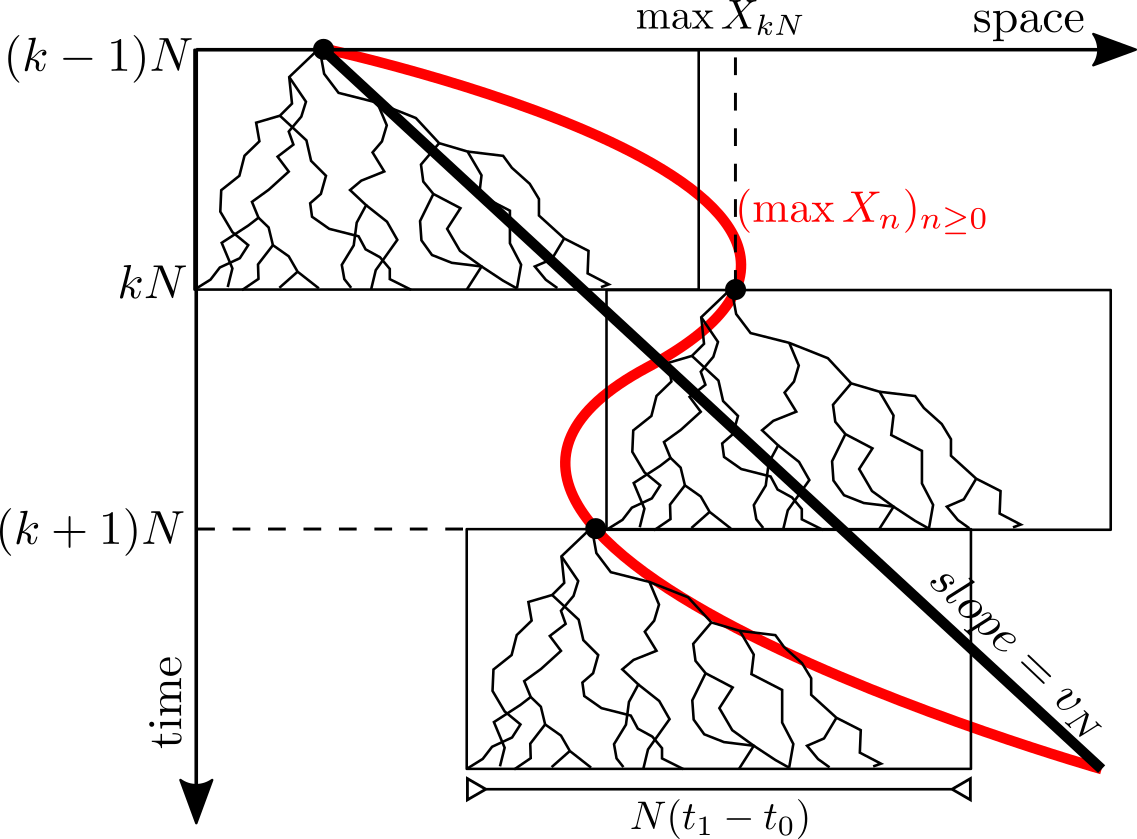
\includegraphics[width=0.8\textwidth]{graphics/g1.png}
% \caption{\label{fig:your-figure}}
\end{figure}

\end{frame}




\begin{frame}{Upper bound on velocity}
\begin{itemize}
\item By Subadditivity $v_N \leq \frac{\E \max X_n}{n}$ for all $n \geq 1$. 
\item Decompose $\E \max X_n$ and prove upper bound on it: 
\begin{align*}
\E \max X_n / n \leq - (1-\gamma)\epsilon + \E \max X_n \Ind_{\max X_n \geq \delta n} \\
+ \delta\, \Pr{\max X_n \geq -(1-\gamma) \epsilon n}
\end{align*}
\end{itemize}

\begin{figure}
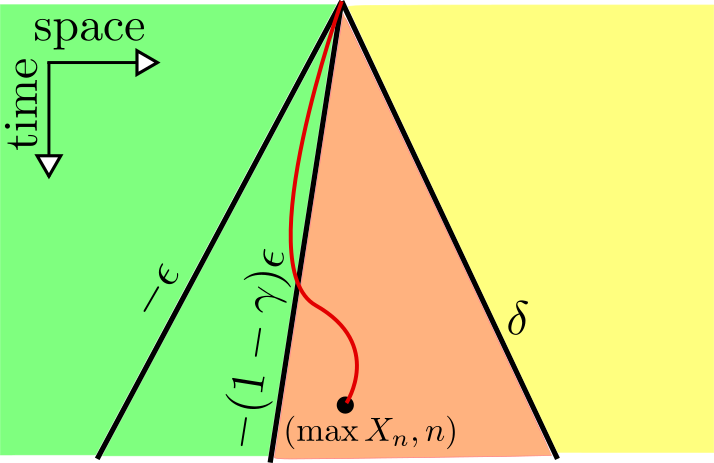
\includegraphics[width=0.8\textwidth]{graphics/decomposition.png}
% \caption{\label{fig:your-figure}}
\end{figure}
\end{frame}

\begin{frame}{Lower bound on velocity}
Comes down to showing $\Pr{\min X_k < -(1+\gamma)n\,\forall\,k \in [n]}$ is small
\begin{figure}
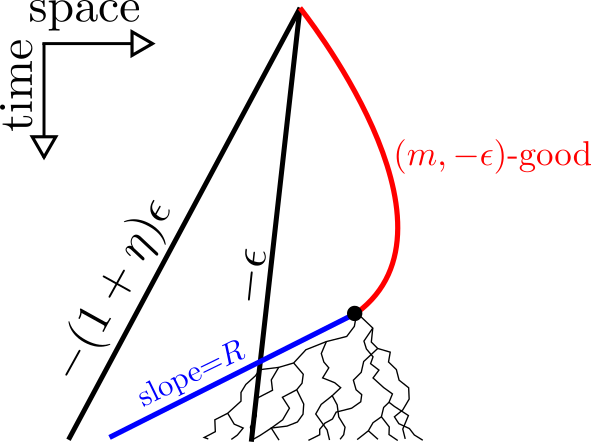
\includegraphics[width=0.8\textwidth]{graphics/lower_bound_proof.png}
% \caption{\label{fig:your-figure}}
\end{figure}
\end{frame}

\begin{frame}{Binary branching, standard normals}
\begin{figure}
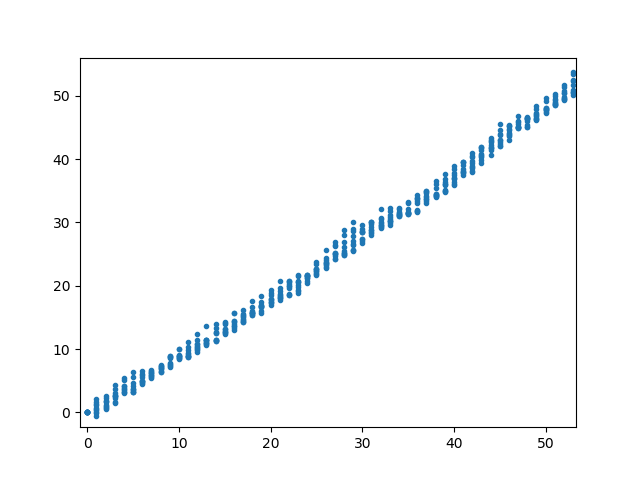
\includegraphics[width=0.8\textwidth]{graphics/std_normal.png}
% \caption{\label{fig:your-figure}}
\end{figure}
\end{frame}

\begin{frame}{Binary branching, Cauchy}
\begin{figure}
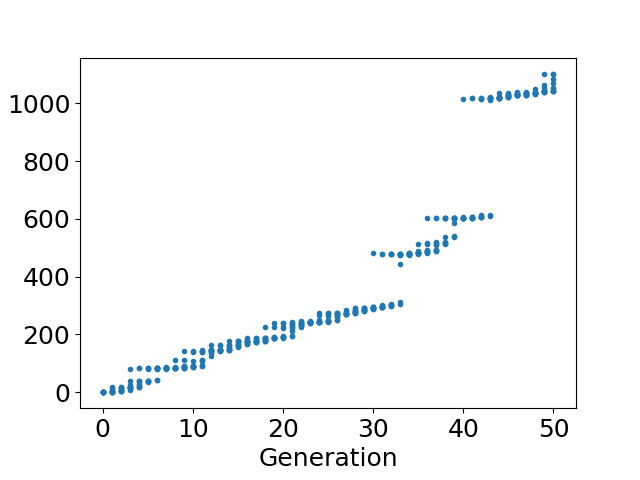
\includegraphics[width=0.8\textwidth]{graphics/cauchy.png}
% \caption{\label{fig:your-figure}}
\end{figure}
\end{frame}

\begin{frame}{$PPP(e^{-x} \nu_\alpha)$}
\begin{figure}
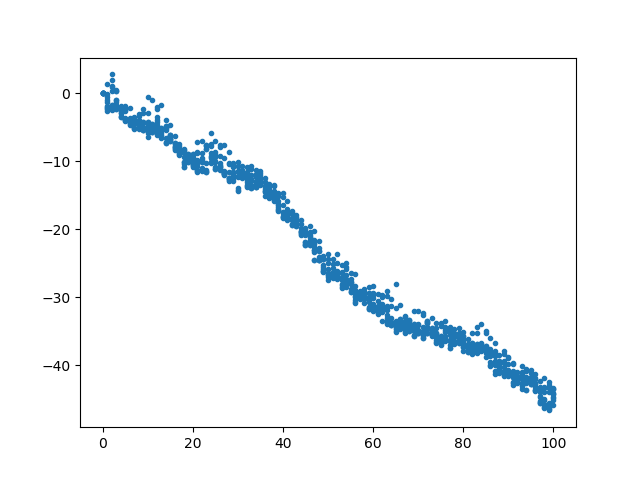
\includegraphics[width=0.8\textwidth]{graphics/cauchy_PPP.png}
% \caption{\label{fig:your-figure}}
\end{figure}
\end{frame}



\section{References}
\bibliographystyle{plain}
\bibliography{bibliography}

\end{document}

% \begin{block}{Examples}
% Some examples of commonly used commands and features are included, to help you get started.
% \end{block}

% Commands to include a figure:
% \begin{figure}
% \includegraphics[width=\textwidth]{your-figure's-file-name}
% \caption{\label{fig:your-figure}Caption goes here.}
% \end{figure}

% \begin{table}
% \centering
% \begin{tabular}{l|r}
% Item & Quantity \\\hline
% Widgets & 42 \\
% Gadgets & 13
% \end{tabular}
% \caption{\label{tab:widgets}An example table.}
% \end{table}
